\begin{surferPage}[Sextica-Barth]{Sextica lui Barth}
    Aceast\u{a} suprafa\c{t}\u{a} de grad $6$ (sextic\u{a}) a fost construit\u{a} de Wolf Barth \^{i}n 1996.
    
    Sextica lui Barth are $65$ de singularit\u{a}\c{t}i \^{i}n total. Acesta este num\u{a}rul maxim posibil 
    de singularit\u{a}\c{t}i ale unei sextice, a\c{s}a cum au demonstrat Jaffe \c{s}i Ruberman, imediat 
    dup\u{a} apari\c{t}ia construc\c{t}iei lui Barth -- deci recordul mondial al lui Barth este de ne\^{i}nvins!
    
   Construc\c{t}ia lui Barth a fost o mare surpriz\u{a}, pentru c\u{a} mult timp s-a crezut c\u{a} suprafe\c{t}ele 
   de grad $6$ pot avea cel mult $64$ de singularit\u{a}\c{t}i.
 
   O caracteristic\u{a} principal\u{a} a construc\c{t}iei este simetria ei icosahedral\u{a}; figura arat\u{a} un 
   icosahedru si planurile lui de simetrie:

  \begin{center}
      \vspace*{-0.1cm}
      \begin{tabular}{@{}c@{\ \ }c@{\,}c@{}}
        \begin{tabular}{@{}c}
          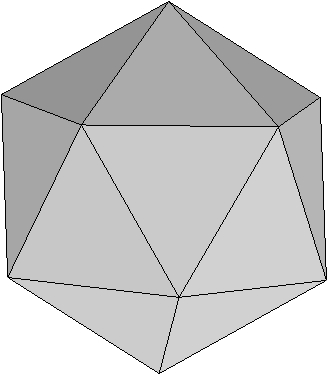
\includegraphics[width=1.4cm]{icosah}
        \end{tabular}
        &
        \begin{tabular}{@{}c}
          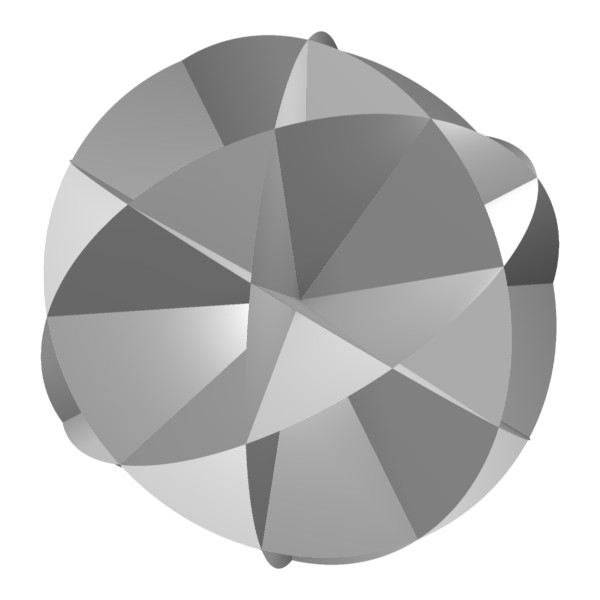
\includegraphics[width=1.4cm]{barth_sextic_planes}
        \end{tabular}
        &
        \begin{tabular}{c@{}}
          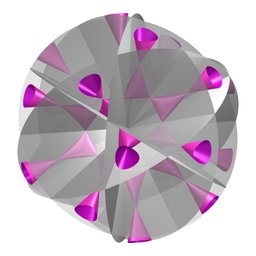
\includegraphics[width=1.4cm]{barth_sextic_and_planes}
        \end{tabular}
      \end{tabular}
    \end{center}
    \vspace*{-0.1cm}

    Sextica lui Barth satisface ecua\c{t}ia $P_6 - \alpha K^2=0,$ unde $P_6$ desemneaz\u{a} cele \c{s}ase
    planuri de simetrie, $K=x^2+y^2+z^2-1$ este sfera unitate \c{s}i $\alpha=\frac{1}{4}(2+\sqrt{5})$.
\end{surferPage}
